\section{Implementation} \label{sec:implementation}
Three systems compromise the project:
\begin{mylist}
  \item The Hardware, Mechanics and Electronics
  \item The software that coordinates the various components
  \item The computer vision system
\end{mylist}

\noindent
It is important to note that the system has undergone significant design changes during its development. The following section
will discuss the final implementation of the system, and a seperate section has been dedicated for discussion on design changes
and problems faced during development that helped inform the final design.
% It is important to note that for the initial version of the system, prior to conducting a comprehensive literature review,
% the system's design incorporated a face-up camera intended to identify components placed on an acrylic plate directly above it.
% This design was chosen as it was the simplest design that would allow for component identification and could 
% be easily implemented using available resources. Additionally, the camera used in the system had 
% a short ribbon cable, which limited the distance between the camera and the Pi. This would have made the face-down
% design more difficult to reasonably immediately implement, especially with the LCD. A longer ribbon cable was ordered
% for this purpose.

% Hardware
\include*{subpages/Hardware}
% Figures for 3D Printed Frame
\begin{figure*}
  \begin{minipage}[t]{0.32\textwidth}
    \centering
    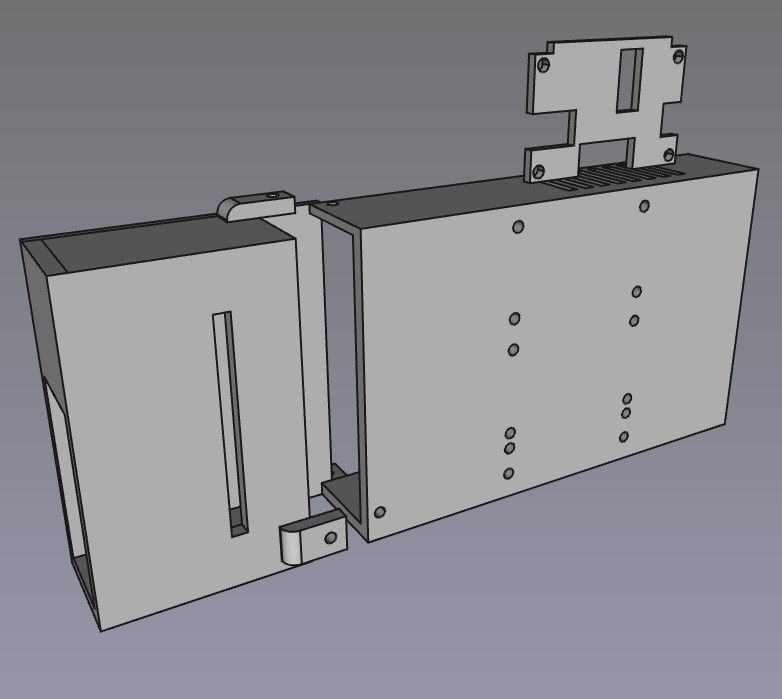
\includegraphics[width=\textwidth,height=5cm]{imgs/freecad/psu_mount.jpg}
    \caption{PSU Housing}
  \end{minipage}
  \hfill
  \begin{minipage}[t]{0.32\textwidth}
    \centering
    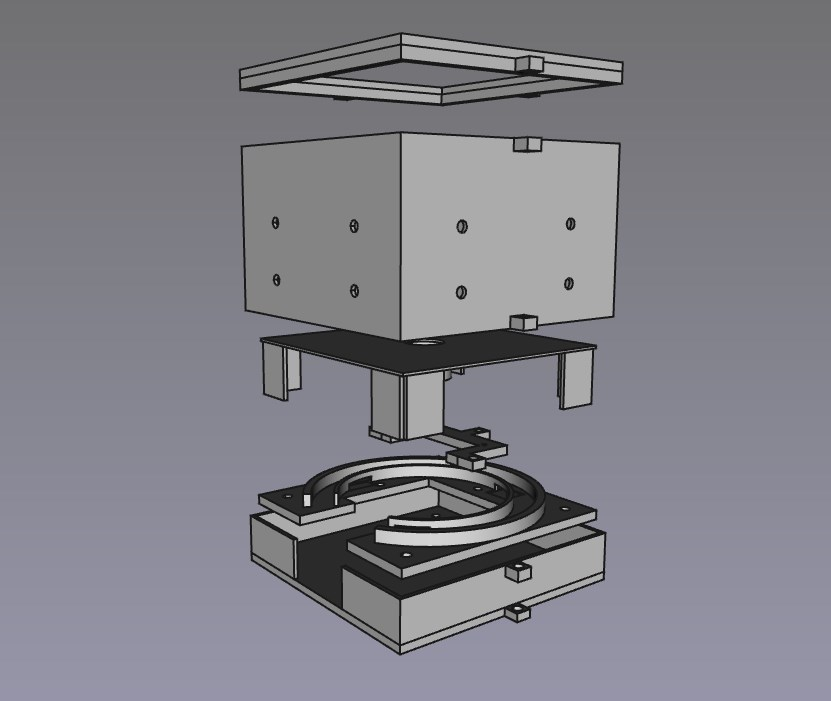
\includegraphics[width=\textwidth,height=5cm]{imgs/freecad/camera_case.jpg}
    \caption{Camera Housing}
    \label{fig:camerahousing}
  \end{minipage}
  \hfill
  \begin{minipage}[t]{0.32\textwidth}
    \centering
    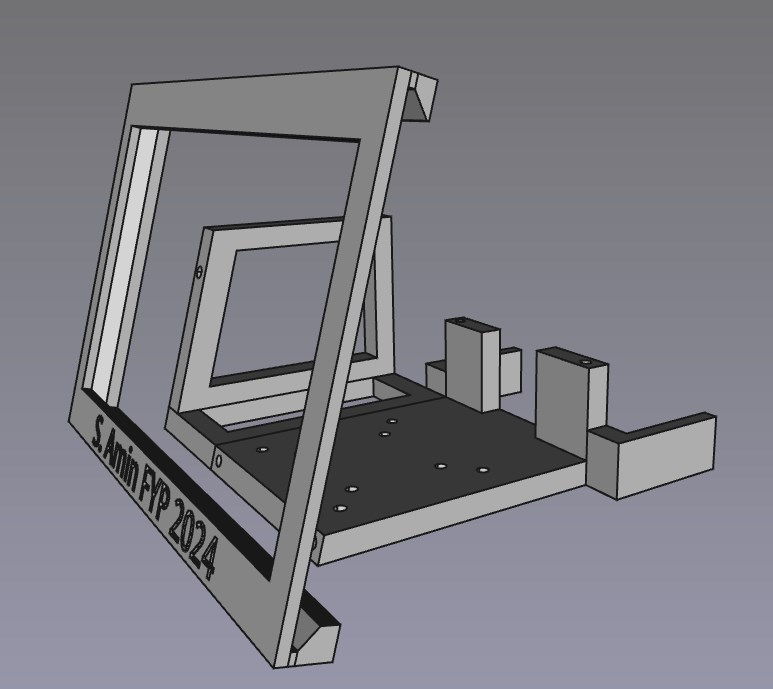
\includegraphics[width=\textwidth,height=5cm]{imgs/freecad/lcd_mount.jpg}
    \caption{LCD Display Housing}
  \end{minipage}
\end{figure*}

% 3D Printed Frame
\include*{subpages/Mechanics}

% Electronics
\include*{subpages/Electronics}

% Software
\include*{subpages/Software}

% Computer Vision
\include*{subpages/Computer Vision}

